% Pre-ambulo
\documentclass[a4paper, 12pt]{abnt}

\usepackage[brazil]{babel}
\usepackage[utf8]{inputenc}
\usepackage[T1]{fontenc}
\usepackage{dsfont}
\usepackage{amssymb,amsmath}
\usepackage{multirow}
\usepackage[alf]{abntcite}
\usepackage[pdftex]{color, graphicx}
\usepackage{colortbl}
\usepackage{url}
\usepackage{abnt-alf}
\usepackage{abntcite}
\usepackage{algorithm}
\usepackage{algorithmic}
%\usepackage{alg}
%\usepackage{hyperref}


% Redefinicao de instrucoes
\floatname{algorithm}{Algoritmo}
\renewcommand{\algorithmicrequire}{\textbf{Entrada:}}
\renewcommand{\algorithmicensure}{\textbf{Saída:}}
\renewcommand{\algorithmicend}{\textbf{fim}}
\renewcommand{\algorithmicif}{\textbf{se}}
\renewcommand{\algorithmicthen}{\textbf{então}}
\renewcommand{\algorithmicelse}{\textbf{senão}}
\renewcommand{\algorithmicfor}{\textbf{para}}
\renewcommand{\algorithmicforall}{\textbf{para todo}}
\renewcommand{\algorithmicdo}{\textbf{faça}}
\renewcommand{\algorithmicwhile}{\textbf{enquanto}}
\renewcommand{\algorithmicloop}{\textbf{loop}}
\renewcommand{\algorithmicrepeat}{\textbf{repetir}}
\renewcommand{\algorithmicuntil}{\textbf{até que}}
\renewcommand{\algorithmiccomment}[1]{\% #1}


% Definicao da lista de simbolos
% \simb[entrada na lista de simbolos]{simbolo}:
% Escreve o simbolo no texto e uma entrada na lista de simbolos.
% Se o parametro opcional e omitido, usa-se o parametro obrigatorio.
\newcommand{\simb}[2][]
{%
	\ifthenelse{\equal{#1}{}}
	{\addcontentsline{los}{simbolo}{#2}}
	{\addcontentsline{los}{simbolo}{#1}}#2
}
% Para aceitar comandos com @ (at) no nome
\makeatletter 
% \listadesimbolos: comando que imprime a lista de simbolos
\newcommand{\listadesimbolos}
{
	\pretextualchapter{Lista de símbolos}
	{\setlength{\parindent}{0cm}
	\@starttoc{los}}
}
% Como a entrada sera impressa
\newcommand\l@simbolo[2]{\par #1}
\makeatother


% Definicao da lista de abreviaturas e siglas
% \abrv[entrada na lista de simbolos]{abreviatura}:
% Escreve a sigla/abreviatura no texto e uma entrada na lista de abreviaturas e siglas.
% Se o parametro opcional e omitido, usa-se o parametro obrigatorio.
\newcommand{\abrv}[2][]
{%
	\ifthenelse{\equal{#1}{}}
	{\addcontentsline{loab}{abreviatura}{#2}}
	{\addcontentsline{loab}{abreviatura}{#1}}#2
}
% Para aceitar comandos com @ (at) no nome
\makeatletter 
% \listadeabreviaturas: comando que imprime a lista de abreviaturas e siglas
\newcommand{\listadeabreviaturas}
{
	\pretextualchapter{Lista de abreviaturas e siglas}
	{\setlength{\parindent}{0cm}
	\@starttoc{loab}}
}
% Como a entrada sera impressa
\newcommand\l@abreviatura[2]{\par #1}
\makeatother


% \listofalgorithms: comando que imprime a lista de algoritmos
\renewcommand{\listalgorithmname}{Lista de algoritmos}


% Hifenização de palavras feita de forma incorreta pelo LaTeX
\hyphenation{PYTHON ou-tros}

\newcommand{\Mautor}{Denis José Sousa de Albuquerque}
\newcommand{\Mtitulo}{Development Issues using SparkSQL}
\newcommand{\Morientador}{Prof. Dr. Umberto Souza da Costa}
\newcommand{\Mdata}{maio de 2018}
\newcommand{\Mlinha}{Programming Languages and Formal Methods}

% Inicio do documento
\begin{document}

	\frenchspacing
	
	% Capa (arquivo Includes/Capa.tex)
	%% Capa
% Proteção externa do trabalho e sobre a qual se imprimem as informações indispensáveis 
% à sua identificação.

% Especificação da capa
\begin{titlepage}
	\begin{center}
		
		% Cabeçalho (não deve ser modificado)
		% Contém o brasão da Universidade, o logotipo do Departamento, além dos dados
		% relacionados à vinculação do aluno (Universidade, Centro, Departamento e Curso)
		\begin{minipage}{2.3cm}
			\begin{center}
				
\includegraphics[width=2.25cm, height=2.68cm]{Imagens/Brasao-UFRN.jpg}
			\end{center}
		\end{minipage}
		\begin{minipage}{11.15cm}
			\begin{center}
				\begin{espacosimples}
					{\small \ \\
                       \textsc{Universidade Federal do Rio Grande do Norte}		   			\\
							  \textsc{Centro de Ciências Exatas e da Terra}					\\
							  \textsc{Departmento de Informática e Matemática Aplicada}	   	\\
							  \textsc{Programa de Pós-Graduação em Sistemas e Computação}  	\\
                       \textsc{Mestrado Acadêmico em Sistemas e Computação}}   				\\
				\end{espacosimples}
			\end{center}
		\end{minipage}
		\begin{minipage}{2.3cm}
			\begin{center}
				
\includegraphics[width=2cm, height=1.96cm]{Imagens/Logotipo-DIMAp.png}
			\end{center}
		\end{minipage}
			
		\vspace{6cm}
						
		% Título do trabalho
		{\setlength{\baselineskip}%
		{1.3\baselineskip}
		{\LARGE \textbf{\Mtitulo}}\par}
			
		\vspace{3cm}
			
		% Nome do aluno (autor)
		{\large \textbf{\Mautor}}
						
		\vspace{6cm}
		
		% Local da instituição onde o trabalho deve ser apresentado e ano de entrega do mesmo
		Natal-RN\\\Mdata
	\end{center}
\end{titlepage}

	% Folha de rosto (arquivo Includes/FolhaRosto.tex)
	%% Folha de rosto
% Contém os elementos essenciais à identificação do trabalho.

% Título, nome do aluno e respectivo orientador e filiação
\titulo{\Large{Título}}
\autor{Nome completo do autor}
\orientador[Orientador]{\par Nome completo do orientador e titulação}
\instituicao
{
	PPgSC -- Programa de Pós-Graduação em Sistemas e Computação\par 
	DIMAp -- Departamento de Informática e Matemática Aplicada\par
   CCET -- Centro de Ciências Exatas e da Terra\par
   UFRN -- Universidade Federal do Rio Grande do Norte
}
	
% Natureza do trabalho (não deve ser modificada)
\comentario
{
	Tese de Doutorado apresentada ao Programa de Pós-Graduação em Sistemas e Computação do Departamento de Informática e Matemática Aplicada da Universidade Federal do Rio Grande do Norte como requisito parcial para a obtenção do grau de Mestre em Sistemas e Computação.\bigskip\\
   \textit{Linha de pesquisa}:\\Nome da linha de pesquisa
}
		
% Local e data
\local{Natal-RN}
\data{Mês e ano}
	
\folhaderosto	
	
	% Folha de aprovacao (arquivo Includes/FolhaAprovacao.tex)
	%% Folha de aprovação
\begin{folhadeaprovacao}
	\setlength{\ABNTsignthickness}{0.4pt}
	\setlength{\ABNTsignwidth}{10cm}
	
	% Informações gerais acerca do trabalho 
	% (nome do autor, título, instituição à qual é submetido e natureza)
	\noindent 
	Tese de Doutorado sob o título \textit{Título} apresentada por Nome completo do autor e aceita pelo Programa de Pós-Graduação em Sistemas e Computação do Departamento de Informática e Matemática Aplicada da Universidade Federal do Rio Grande do Norte, sendo aprovada por todos os membros da banca examinadora abaixo especificada:
		
	% Membros da banca examinadora e respectivas filiações
	\assinatura
	{
		Nome completo do orientador e titulação   			                  \\
		{\small Presidente}											          \smallskip\\ 
		{\footnotesize
			DIMAp -- Departamento de Informática e Matemática Aplicada		   \\
		  	UFRN -- Universidade Federal do Rio Grande do Norte
		}
   }
      
   \assinatura
	{
      Nome completo do examinador e titulação   			                  \\
		{\small Examinador}											          \smallskip\\ 
		{\footnotesize
			Departamento		\\
		  	Universidade
		}
   }   
   
   \assinatura
	{
      Nome completo do examinador e titulação   			                  \\
		{\small Examinador}											          \smallskip\\ 
		{\footnotesize
			Departamento		\\
		  	Universidade
		}
	}
		
	\vfill
	
	\begin{center}
		Natal-RN, data da defesa (dia, mês e ano).
	\end{center}
\end{folhadeaprovacao}
	
	
	% Dedicatoria (arquivo Includes/Dedicatoria.tex)
	%% Dedicatória

\chapter*{}
\vspace{15cm}
\begin{flushright}
	Homenagem que o autor presta a uma ou mais pessoas.
\end{flushright}
	
	% Agradecimentos (arquivo Includes/Agradecimentos.tex)
	%% Agradecimentos

\chapter*{Agradecimentos}

Agradecimentos dirigidos àqueles que contribuíram de maneira relevante à elaboração do trabalho, sejam eles pessoas ou mesmo organizações.
   
   % Epigrafe (arquivo Includes/Epigrafe.tex)
	%% Epígrafe (citação seguida de indicação de autoria)

\chapter*{}
\vspace{15cm}
\begin{flushright}
	\textit
	{
		Citação
	}\medskip\\ 
	Autor
\end{flushright}
	
	% Resumo em língua vernacula (arquivo Includes/Resumo.tex)
	%% Resumo em língua vernácula
\begin{center}
	{\Large{\textbf{Título do trabalho}}}
\end{center}

\vspace{1cm}

\begin{flushright}
	Autor: Nome do aluno\\
	Orientador(a): Titulação e nome do(a) orientador(a)
\end{flushright}

\vspace{1cm}

\begin{center}
	\Large{\textsc{\textbf{Resumo}}}
\end{center}

\noindent O resumo deve apresentar de forma concisa os pontos relevantes de um texto, fornecendo uma visão rápida e clara do conteúdo e das conclusões do trabalho. O texto, redigido na forma impessoal do verbo, é constituído de uma seqüência de frases concisas e objetivas e não de uma simples enumeração de tópicos, não ultrapassando 500 palavras, seguido, logo abaixo, das palavras representativas do conteúdo do trabalho, isto é, palavras-chave e/ou descritores. Por fim, deve-se evitar, na redação do resumo, o uso de parágrafos (em geral resumos são escritos em parágrafo único), bem como de fórmulas, equações, diagramas e símbolos, optando-se, quando necessário, pela transcrição na forma extensa, além de não incluir citações bibliográficas.

\noindent\textit{Palavras-chave}: Palavra-chave 1, Palavra-chave 2, Palavra-chave 3.
	
	% Abstract, resumo em língua estrangeira (arquivo Include/Abstract.tex)
	%% Resumo em língua estrangeira (em inglês Abstract, em espanhol Resumen, em francês Résumé)
\begin{center}
	{\Large{\textbf{Título do trabalho (em língua estrangeira)}}}
\end{center}

\vspace{1cm}

\begin{flushright}
	Author: Nome do aluno\\
	Supervisor: Titulação e nome do(a) orientador(a)
\end{flushright}

\vspace{1cm}

\begin{center}
	\Large{\textsc{\textbf{Abstract}}}
\end{center}

\noindent O resumo em língua estrangeira (em inglês \textit{Abstract}, em espanhol \textit{Resumen}, em francês \textit{Résumé}) é uma versão do resumo escrito na língua vernácula para idioma de divulgação internacional. Ele deve apresentar as mesmas características do anterior (incluindo as mesmas palavras, isto é, seu conteúdo não deve diferir do resumo anterior), bem como ser seguido das palavras representativas do conteúdo do trabalho, isto é, palavras-chave e/ou descritores, na língua estrangeira. Embora a especificação abaixo considere o inglês como língua estrangeira (o mais comum), não fica impedido a adoção de outras linguas (a exemplo de espanhol ou francês) para redação do resumo em língua estrangeira.

\noindent\textit{Keywords}: Keyword 1, Keyword 2, Keyword 3.
	
	% Lista de figuras
	%\listoffigures

	% Lista de tabelas
	%\listoftables
	
	% Lista de abreviaturas e siglas
	%\listadeabreviaturas
	
	% Lista de símbolos
	%\listadesimbolos
	
	% Lista de algoritmos (se houver)
	% Devem ser incluídos os pacotes algorithm e algorithmic
	% \listofalgorithms
	
	% Sumário
	\sumario

	% Introdução
\chapter{Introduction}

The current volume of data available on the Internet has led to new opportunities and challenges. The processing of Big Data is often done on a distributed environment, since processing a huge amount of data exceeds the capabilities of single machines. In this scenario the developer has to manage the complexity of the data partitioning, the distribution of the computation and a much more complex failure handling.

Several research efforts has been done in order help developers to deal with the complexity of distributed systems. This help often take the form of middleware or programming frameworks \cite{ranganathan2007complexity}. One of these initiatives is Apache Spark~\footnote{https://spark.apache.org/}. It was released in 2010 and has been adopted by many industries, being the most active open source project for big data processing \cite{armbrust2015sparksql}. 

Spark is a cluster computing framework for implementing large-scale data processing applications while providing scalability and fault tolerance \cite{zaharia2010spark}. To use Spark, developers write a program that implements the high-level control flow of their application. The control flow is specified by using one of the supported programming language (Java, Scala, Python, R or SQL) and libraries for extended functionalities. These libraries includes Spark SQL for relational data, MLib for  machine learning, GraphX for graph processing, as well as a library for stream processing.

As stated by \cite{ranganathan2007complexity}, developers often face steep learning curves before they can start programming large distributed systems. The use of well-known technologies can help reduce this effort because developers will be able to reuse the knowledge they once learned and a lot of educational documentation has been produced already.

In the context of data processing, the use of SQL and the Relational Database Management Systems is plentiful. They have proven their worth over the years. The popularity of SQL shows that developers often prefer writing declarative queries to deal with data. But, according to \cite{armbrust2015sparksql} the relational-only approach is insufficient for many big data applications, such as those who deal with machine learning and graph processing.

Spark SQL aims to combine both declarative relational queries and imperative procedural algorithms. It extends Spark with a declarative API in order to provide an integrated and easy-to-use environment for big Data. According to \cite{armbrust2015sparksql}, users feedback and benchmarks show that Spark SQL makes it significantly simpler and more efficient to write data pipelines that mix relational and procedural processing. 

Nevertheless, the coding of a Spark SQL application is not a trivial task.
To better understand the problems often encountered by programmers when developing big data processing applications with Spark SQL, this research proposes the identification and classification of these problems.

\section{Motivation}

Several researches were conducted to identify difficulties faced by software developers (TODO: Incluir Referências). But, to our knowledge, there are no studies that focused on get insights into the obstacles encountered by programmers in the domain of big data. This work aims to help filling this gap by identifying the problems faced by Spark SQL applications developers.

The results of such analysis could improve the current situation as a first step to empower the Spark application developer with a better toolset.  For instance, it could be used to construct development practice guidelines, automated test cases generation or tools for static analysis of code.

To do this work, it is important that it be conducted with as much organization as possible. Taxonomy is a key tool for this organization inasmuch its hierarchical structure provides a way to classify the knowledge for a fast retrieval of information.

The development of a taxonomy of errors in application development could be one key step to systematically address and resolve the problems identified. Such taxonomy may be developed to categorize the types of errors, to explain why a specific error occurs, and to generate intervention strategies for each type of error.

\section{General Goal}

The main goal of this work is to construct a taxonomy of errors related to the development of big data processing applications with Spark SQL.

\section{Specific Goals}

This work aims to address the following research questions:

\begin{enumerate}
    \item Which are the difficulties that developers often face when implementing Spark SQL applications?
    
    \item Is the pattern of errors usually faced by Spark SQL developers the same one faced by SQL developers who works with other platforms?
    
    SQL is used as interface for many database management systems (DBMS), including Spark SQL. Here we want to identify the similarities and differences in problems found in the Spark SQL and other DBMS. 
    
    \item How the API notation changes the pattern of implementation errors when compared to SQL standard statements?
    
\end{enumerate}

With the first question we seek to identify the kinds of problems found, why these problems happens and how they are resolved. 

SQL is used as interface for many systems, including Spark SQL. With the second question  we want to identify the similarities and differences in problems found in the Spark SQL and in Database Management Systems.

In addition to raw SQL commands, the Spark SQL application developer can also use an functional API to deal with the relational data. Answering the third question we want to identify if the problems are related to the notation used.
    
\section{The Problem Scope}

The domain of big data applications is wide. For the purpose of this work, the analysis will be restricted to Spark SQL applications.

\section{Contributions}

\section{Thesis Organization}

The remainder of this thesis is organized as follows. In Chapter ...
	% % Capítulo 2
\chapter{Background}

Este é o primeiro capítulo da parte central do trabalho, isto é, o desenvolvimento, a parte mais extensa de todo o trabalho. Geralmente o desenvolvimento é dividido em capítulos, cada um com subseções e subseções, cujo tamanho e número de divisões variam em função da natureza do conteúdo do trabalho.

Em geral, a parte de desenvolvimento é subdividida em quatro subpartes:

\begin{itemize}
   \item \textit{contextualização ou definição do problema} -- consiste em descrever a situação ou o contexto geral referente ao assunto em questão, devem constar informações atualizadas visando a proporcionar maior consistência ao trabalho;
   \item \textit{referencial ou embasamento teórico} -- texto no qual se deve apresentar os aspectos teóricos, isto é, os conceitos utilizados e a definição dos mesmos; nesta parte faz-se a revisão de literatura sobre o assunto, resumindo-se os resultados de estudos feitos por outros autores, cujas obras citadas e consultadas devem constar nas referências;
   \item \textit{metodologia do trabalho ou procedimentos metodológicos} -- deve constar o instrumental, os métodos e as técnicas aplicados para a elaboração do trabalho;
   \item \textit{resultados} -- devem ser apresentados, de forma objetiva, precisa e clara, tanto os resultados positivos quanto os negativos que foram obtidos com o desenvolvimento do trabalho, sendo feita uma discussão que consiste na avaliação circunstanciada, na qual se estabelecem relações, deduções e generalizações.
\end{itemize}

É recomendável que o número total de páginas referente à parte de desenvolvimento não ultrapasse 60 (sessenta) páginas.

\section{Spark}

Teste de figura:

\begin{figure}[htb]
	\centering
  	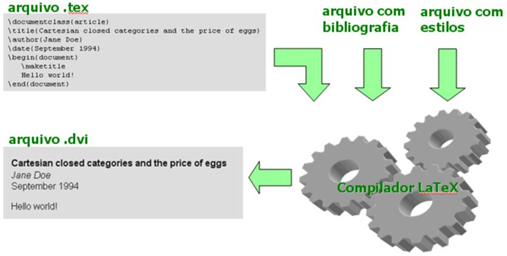
\includegraphics[scale=0.75]{Imagens/FiguraTeste.png}
  	\textsf{\caption{Teste de uma figura em formato .png}}
  	\label{fig:FiguraTeste}
\end{figure}


\section{Stackoverflow}

Referenciamento da figura inserida na seção anterior: \ref{fig:FiguraTeste}

	% % Capítulo 4
\chapter{Related Works}

Teste para abreviatura 

\abrv[UFRN -- Universidade Federal do Rio Grande do Norte]{UFRN}

\abrv[DIMAp -- Departamento de Informática e Matemática Aplicada]{DIMAp}
	% % Capítulo 3
\chapter{The Proposal}

Algumas regras devem ser observadas na redação da dissertação/tese: 

\begin{itemize}
   \item ser claro, preciso, direto, objetivo e conciso, utilizando frases curtas e evitando ordens inversas desnecessárias;
   \item construir períodos com no máximo duas ou três linhas, bem como parágrafos com cinco linhas cheias, em média, e no máximo oito (ou seja, não construir parágrafos e períodos muito longos, pois isso cansa o(s) leitor(es) e pode fazer com que ele(s) percam a linha de raciocínio desenvolvida);
   \item a simplicidade deve ser condição essencial do texto; a simplicidade do texto não implica necessariamente repetição de formas e frases desgastadas, uso exagerado de voz passiva (como \textit{será iniciado}, \textit{será realizado}), pobreza vocabular etc. Com palavras conhecidas de todos, é possível escrever de maneira original e criativa e produzir frases elegantes, variadas, fluentes e bem alinhavadas;
   \item adotar como norma a ordem direta, por ser aquela que conduz mais facilmente o leitor à essência do texto, dispensando detalhes irrelevantes e indo diretamente ao que interessa, sem ``rodeios'' (verborragias);
   \item não começar períodos ou parágrafos seguidos com a mesma palavra, nem usar repetidamente a mesma estrutura de frase;
   \item desprezar as longas descrições e relatar o fato no menor número possível de palavras;
   \item recorrer aos termos técnicos somente quando absolutamente indispensáveis e nesse caso colocar o seu significado entre parênteses (ou seja, não se deve admitir que todos os que lerão o trabalho já dispõem de algum conhecimento desenvolvido no mesmo);
   \item dispensar palavras e formas empoladas ou rebuscadas, que tentem transmitir ao leitor mera ideia de erudição (até mesmo às vezes ilusória);
   \item não perder de vista o universo vocabular do leitor, adotando a seguinte regra prática: \textit{nunca escrever o que não se diria};
   \item termos coloquiais ou de gíria devem ser usados com extrema parcimônia (ou mesmo nem serem utilizados) e apenas em casos muito especiais, para não darem ao leitor a ideia de vulgaridade e descaracterizar o trabalho;
   \item ser rigoroso na escolha das palavras do texto, desconfiando dos sinônimos perfeitos ou de termos que sirvam para todas as ocasiões; em geral, há uma palavra para definir uma situação;
   \item encadear o assunto de maneira suave e harmoniosa, evitando a criação de um texto onde os parágrafos se sucedem uns aos outros como compartimentos estanques, sem nenhuma fluência entre si;
   \item ter um extremo cuidado durante a redação do texto, principalmente com relação às regras gramaticais e ortográficas da língua; geralmente todo o texto é escrito na forma impessoal do verbo, não se utilizando, portanto, de termos em primeira pessoa, seja do plural ou do singular.
\end{itemize}

Continuação do texto.


\section{The Proposed Method}

Teste de tabela.

\begin{table}[!htb]
   \textsf{\caption{Tabela sem sentido.}}
   \centering
   \medskip
   \begin{tabular}{c|p{6cm}}
      \hline
      \textbf{Título Coluna 1} & \textbf{Título Coluna 2} \\
      \hline
      Texto curto & Texto mais extenso, que requer mais de uma linha \\
      \hline
      \label{tab:TabelaSemSentido}
   \end{tabular}
\end{table}


\section{Next Steps}

Seção 2


\subsection{Subseção 2.1}

Referência à tabela definida no início: \ref{tab:TabelaSemSentido}


\subsection{Subseção 2.2}

Texto a ser enumerado.

\begin{enumerate}
   \item Item 1
   \item Item 2, com nota explicativa\footnote{Nota explicativa}
   \item Item 3
\end{enumerate}


\section{Schedule}

Texto antes de equação.

\begin{equation}
   x = y + z
\end{equation}

Texto depois de equação.
	
	% Capitulo 4: Quarto capítulo (arquivo Includes/Capitulo4.tex)
	%% Capítulo 4
\chapter{Capítulo 4}

\section{Seção 1}

Teste para símbolo

\simb[$\lambda$ (algum símbolo)]{$\lambda$}


\section{Seção 2}

Teste para abreviatura 

\abrv[UFRN -- Universidade Federal do Rio Grande do Norte]{UFRN}

\abrv[DIMAp -- Departamento de Informática e Matemática Aplicada]{DIMAp}
	
	% Capitulo 5: Quinto capítulo (arquivo Includes/Capitulo5.tex)
	%% Capítulo 5
\chapter{Capítulo 5}

\section{Seção 1}

Seção 1


\section{Seção 2}

Alguns exemplos de citação: 

Na tese de Doutorado de Paquete \cite{PaquetePhD}, discute-se sobre algoritmos de busca local estocásticos aplicados a problemas de Otimização Combinatória considerando múltiplos objetivos. Por sua vez, o trabalho de \cite{KnowlesBoundedLebesgue}, publicado nos anais do IEEE CEC de 2003, mostra uma técnica de arquivamento também empregada no desenvolvimento de algoritmos evolucionários multi-objetivo, trabalho esse posteriormente estendido para um capítulo de livro dos mesmos autores \cite{KnowlesBoundedPareto}. Por fim, no relatório técnico de \citeonline{Jaszkiewicz}, fala-se sobre um algoritmo genético híbrido para problemas multi-critério, enquanto no artigo de jornal de Lopez \textit{et al.} \cite{LopezPaqueteStu} trata-se do \textit{trade-off} entre algoritmos genéticos e metodologias de busca local, também aplicados no contexto multi-critério e relacionado de alguma forma ao trabalho de Jaszkiewicz (\citeyear{Jaszkiewicz}).

Outros exemplos relacionados encontram-se em \cite{Silberschatz} (livro), \cite{DB2XML} (referência da Web) e \cite{Angelo} (dissertação de Mestrado).

\subsection{Subseção 5.1}

Subseção 5.1


\subsection{Subseção 5.2}

Subsection 5.2


\section{Seção 3}

Seção 3
		
	% Consideracoes finais
	%% Considerações finais
\chapter{Considerações finais}

As considerações finais formam a parte final (fechamento) do texto, sendo dito de forma resumida (1) o que foi desenvolvido no presente trabalho e quais os resultados do mesmo, (2) o que se pôde concluir após o desenvolvimento bem como as principais contribuições do trabalho, e (3) perspectivas para o desenvolvimento de trabalhos futuros, como listado nos exemplos de seção abaixo. O texto referente às considerações finais do autor deve salientar a extensão e os resultados da contribuição do trabalho e os argumentos utilizados estar baseados em dados comprovados e fundamentados nos resultados e na discussão do texto, contendo deduções lógicas correspondentes aos objetivos do trabalho, propostos inicialmente.


\section{Principais contribuições}

Texto.


\section{Limitações}

Texto.


\section{Trabalhos futuros}

Texto.
	
	% Bibliografia (arquivo Capitulos/Referencias.bib)
	\bibliography{Parts/References}
	\bibliographystyle{abnt-alf}
	
	% Apêndice A (arquivo Includes/ApendiceA)
	%% Apêndice
\apendice
\chapter{Primeiro apêndice}

Os apêndices são textos ou documentos elaborados pelo autor, a fim de complementar sua argumentação, sem prejuízo da unidade nuclear do trabalho.
	
	% Anexo A (arquivo Includes/AnexoA)
	%% Anexo
\anexo
\chapter{Primeiro anexo}

Os anexos são textos ou documentos não elaborado pelo autor, que servem de fundamentação, comprovação e ilustração.
	
	% Página em branco
	\newpage

\end{document}